\section{Overview of KIDs}
\label{sec2}
%Brief description of the main features of KIDS. Only those relevant to this work.

Kinetic inductance detectors are a novel superconducting detectors technology that provides high sensitivity and ease of multiplexing. In this section we give a brief summary of the main features of KIDs.\\
KIDs are RLC superconducting resonators made from a thin thin metal films that react with an incoming radiation by changing their electromagnetic properties. In fact, when photons are absorbed by the superconducting film, they break Cooper pairs and change the ratio of paired (Cooper pair) and unpaired (quasi-particles) charge carriers. The breaking of Cooper pairs increases the quasi-particles density, which causes a change in the kinetic inductance $L_{k}$. Therefore, this produces a shift of the resonant frequency of the KID \citep{2013A&A...551L..12C}. The absorbed optical power $P_{opt}$ can be directly related to the change in the resonant frequency $\delta f_{0}$, as the relationship between them is linear for small variations in $P_{opt}$ \citep{2010ApPhL..96z3511S}. The operating principle is represented in fig \ref{resonance}.\\

\begin{figure}[h]
\center
	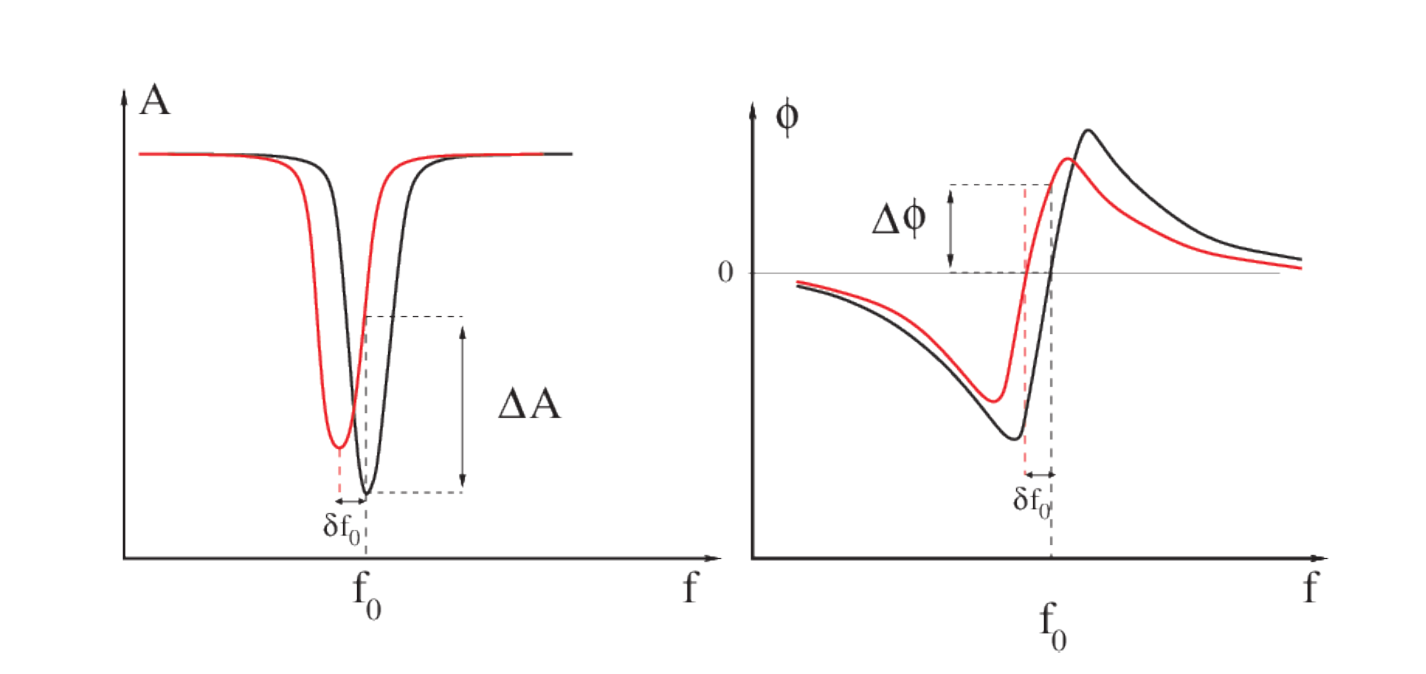
\includegraphics[scale=0.35]{resonance.png}
	\caption{Schematic representation of a KID resonance in amplitude (left) and phase (right), as a function of the excited tone injected in the feedline. The optical power absorbed by the detector is weak for black curves and increases for red curves. The absorption of a photon shifts the resonance frequency and this is directly proportional to the power received.}
	\label{resonance}
\end{figure}

To be able to read a KID circuit, the detector must be coupled with a transmission feedline. The transmission is expressed by the $S_{21}$ parameter which represents the transfer function of the signal measured. 

\begin{equation}
S_{21}(f) = I +jQ
\end{equation}

where I and Q give respectively the real (in phase) and imaginary (quadrature) part of the ratio between the input and output signal of the feedline transmission. \\

Using the circuit model, the complex scattering parameter $S_{21}$ can be calculate following the parametrisation proposed by \citet{2008ApPhL..93m4102G} :

\begin{equation}
S_{21} = \frac{2Z_{res}Z_{0}}{Z_{res}[2Z_{0} + j(X_{1}+X_{2})] + (Z_{0} +jX_{1})(Z_{0} +jX_{2})}
\end{equation}

with :

\begin{equation}
Z_{res} = \frac{Z_{0}Q_{e}}{2Q_{i}}[1 + 2jQ_{i}\frac{(f-f_{0})}{f_{0}}]
\end{equation}

Where $X_{1}$, $X_{2}$, $Z_{0}$ are impedances, $Q_{i}$ is the intrinsic quality factor of the resonator and $Q_{e}$ is the external quality factor due to coupling with the measurement electronics. $f$ is the frequency of excitation to which the detector is submitted, and $f_{0}$ represents the resonant frequency. In this paper we simulate the response of a KID using this parametrisation as presented in the following section.


 


